\documentclass{article}

\usepackage{microtype}
\usepackage{graphicx}
\usepackage{subfigure}
\usepackage{booktabs} % NOTE: for professional tables
\usepackage{makecell}
\usepackage{listings}
\usepackage{xcolor}
\lstset{
  breaklines=true,              % NOTE: enable automatic line breaking
  basicstyle=\small\ttfamily,   % NOTE: adjust the font size and type
  escapeinside={||},            % NOTE: define escape characters for LaTeX commands
}
\usepackage{fancyvrb}
\usepackage{minted}
% Set options for minted:
\setminted{
  breaklines=true,   % Enable automatic line breaking
  fontsize=\small,   % Adjust the font size if needed
  escapeinside=||,
  % Any other options you need
}
\usepackage{mdframed}


\usepackage{lipsum}
\usepackage{listings}
% Rename "Listing: " to "Extract: "
\renewcommand{\lstlistingname}{Extract}

\usepackage{hyperref}


% NOTE: make hyperref and algorithmic work together better:
\newcommand{\theHalgorithm}{\arabic{algorithm}}

% \usepackage{icml2025} % NOTE: will display the line numbers
\usepackage[accepted]{./settings/icml2025} % NOTE: won't display the line numbers
% \usepackage[nohyperref, accepted]{icml2025} % NOTE: won't display the line numbers

% For theorems and such
\usepackage{amsmath}
\usepackage{amssymb}
\usepackage{mathtools}
\usepackage{amsthm}

% if you use cleveref..
\usepackage[capitalize,noabbrev]{cleveref}

%%%%%%%%%%%%%%%%%%%%%%%%%%%%%%%%
% THEOREMS
%%%%%%%%%%%%%%%%%%%%%%%%%%%%%%%%
\theoremstyle{plain}
\newtheorem{theorem}{Theorem}[section]
\newtheorem{proposition}[theorem]{Proposition}
\newtheorem{lemma}[theorem]{Lemma}
\newtheorem{corollary}[theorem]{Corollary}
\theoremstyle{definition}
\newtheorem{definition}[theorem]{Definition}
\newtheorem{assumption}[theorem]{Assumption}
\theoremstyle{remark}
\newtheorem{remark}[theorem]{Remark}

% TODO: is useful during development; simply uncomment the next line
%    and comment out the line below the next line to turn off comments
%\usepackage[disable,textsize=tiny]{todonotes}
\usepackage[textsize=tiny]{todonotes}

\usepackage{multirow}
\usepackage{multicol}
\usepackage{enumitem}
% c.f. Efficient Online Reinforcement Learning Fine-Tuning Need Not Retain Offline Data
\usepackage[most,skins,theorems]{tcolorbox}
\tcbset{
  aibox/.style={
    width=\linewidth,
    top=8pt,
    bottom=4pt,
    colback=blue!6!white,
    colframe=black,
    colbacktitle=black,
    enhanced,
    center,
    attach boxed title to top left={yshift=-0.1in,xshift=0.15in},
    boxed title style={boxrule=0pt,colframe=white,},
  }
}

\newtcolorbox{AIbox}[2][]{aibox,title=#2,#1}

\begin{document}

\twocolumn[
    \icmltitle{Bouldering Video Segmentation \\ \textit{M1 DS Research Project}}

    \icmlsetsymbol{equal}{*}

    \begin{icmlauthorlist}
    \icmlauthor{Nadir Kichou}{ul}
    \icmlauthor{Jérémie Boulanger}{sigma}
    \icmlauthor{Ludivine Plumhans}{ur}
    \icmlauthor{Ludovic Seifert}{ur}
    \end{icmlauthorlist}

    \icmlaffiliation{ul}{Université de Lille}
    \icmlaffiliation{sigma}{CRIStAL Lab, SIGMA}
    \icmlaffiliation{ur}{Université de Rouen}

    \icmlcorrespondingauthor{Nadir Kichou }{nadir.kichou.etu@univ-lille.fr}

    \icmlkeywords{Temporal Action Segmnetation, TAS, Video Machine Learning, Machine Learning, ICML}

    \vskip 0.3in
]

\begin{abstract}
Scaling \todo{Hellow world \ldots} inference compute enhances reasoning in large language models (LLMs), with long chains-of-thought (CoTs) enabling strategies like backtracking and error correction. Reinforcement learning (RL) has emerged as a crucial method for developing these capabilities, yet the conditions under which long CoTs emerge remain unclear, and RL training requires careful design choices. In this study, we systematically investigate the mechanics of long CoT reasoning, identifying the key factors that enable models to generate long CoT trajectories. Through extensive supervised fine-tuning (SFT) and RL experiments, we present four main findings: (1) While SFT is not strictly necessary, it simplifies training and improves efficiency; (2) Reasoning capabilities tend to emerge with increased training compute, but their development is not guaranteed, making reward shaping crucial for stabilizing CoT length growth; (3) Scaling verifiable reward signals is critical for RL. We find that leveraging noisy, web-extracted solutions with filtering mechanisms shows strong potential, particularly for out-of-distribution (OOD) tasks such as STEM reasoning; and (4) Core abilities like error correction are inherently present in base models, but incentivizing these skills effectively for complex tasks via RL demands significant compute, and measuring their emergence requires a nuanced approach. These insights provide practical guidance for optimizing training strategies to enhance long CoT reasoning in LLMs. Our code is available at: \href{https://github.com/eddycmu/demystify-long-cot}{https://github.com/eddycmu/demystify-long-cot}.
\end{abstract}

\section{Introduction}

Here we are going to provide the essential background information.

\todo[inline]{This section might be removed as since we are in report mode and not research mode, we might not need to provide the background information or at least not this early in the report.}

\todo[inline]{Talk about the fact that the data quality is the most important thing and maybe even more important than the model architecture and size and dataset size.}

\todo[inline]{Maybe merge this section with the context.}
\section{Context}
\label{section:context}

\noindent\textbf{Bouldering Basics.} 
It is a form of rock climbing where climbers tackle short but challenging routes, typically lasting around 4 minutes. During this time, climbers have the freedom to choose their climbing strategies, retry as many times as needed, and aim to complete the route as quickly as possible. The ultimate goal is to reach the top of the climb in the least amount of time.

\noindent\textbf{Project Overview.} 
This research project is part of a larger initiative (ANR) aimed at improving bouldering performance. The focus is on developing tools for coaches to analyze bouldering performances, allowing them to provide better advice to help climbers improve.

\noindent\textbf{Existing Tools.} 
Among these tools are: Grip Detection, Path Tracking, Performance Analysis, and more. Several models have already been developed as part of this broader effort, including a model for detecting the grips used by the climber and another for tracking the climber's path during a climb.

\noindent\textbf{Phase Identification.} 
These models provide valuable data, but in order to fully analyze a climber's performance, it is essential to distinguish between the different phases of a bouldering event (Climbing, Observing, Brushing). By doing so, we can apply the appropriate model to each phase and gather the corresponding statistics.

\noindent\textbf{Research Focus.} 
This brings us to my current research project. I will be focusing on Temporal Action Segmentation (TAS), a technique that will allow us to run the grip and path analysis models at the correct timestamps. This step is crucial for gaining deeper insights into the different phases of climbing, such as observing, reading the route, and brushing the grips. By analyzing the durations, order, and impact of these phases on a climber's final performance, we can provide more precise guidance to coaches and improve training methods.

\begin{figure*}[t]
    \centering
    \begin{tabular}{@{}c@{\hspace{15pt}}c@{\hspace{15pt}}c@{\hspace{15pt}}c@{}}
      \setlength{\fboxsep}{0pt}
      \fbox{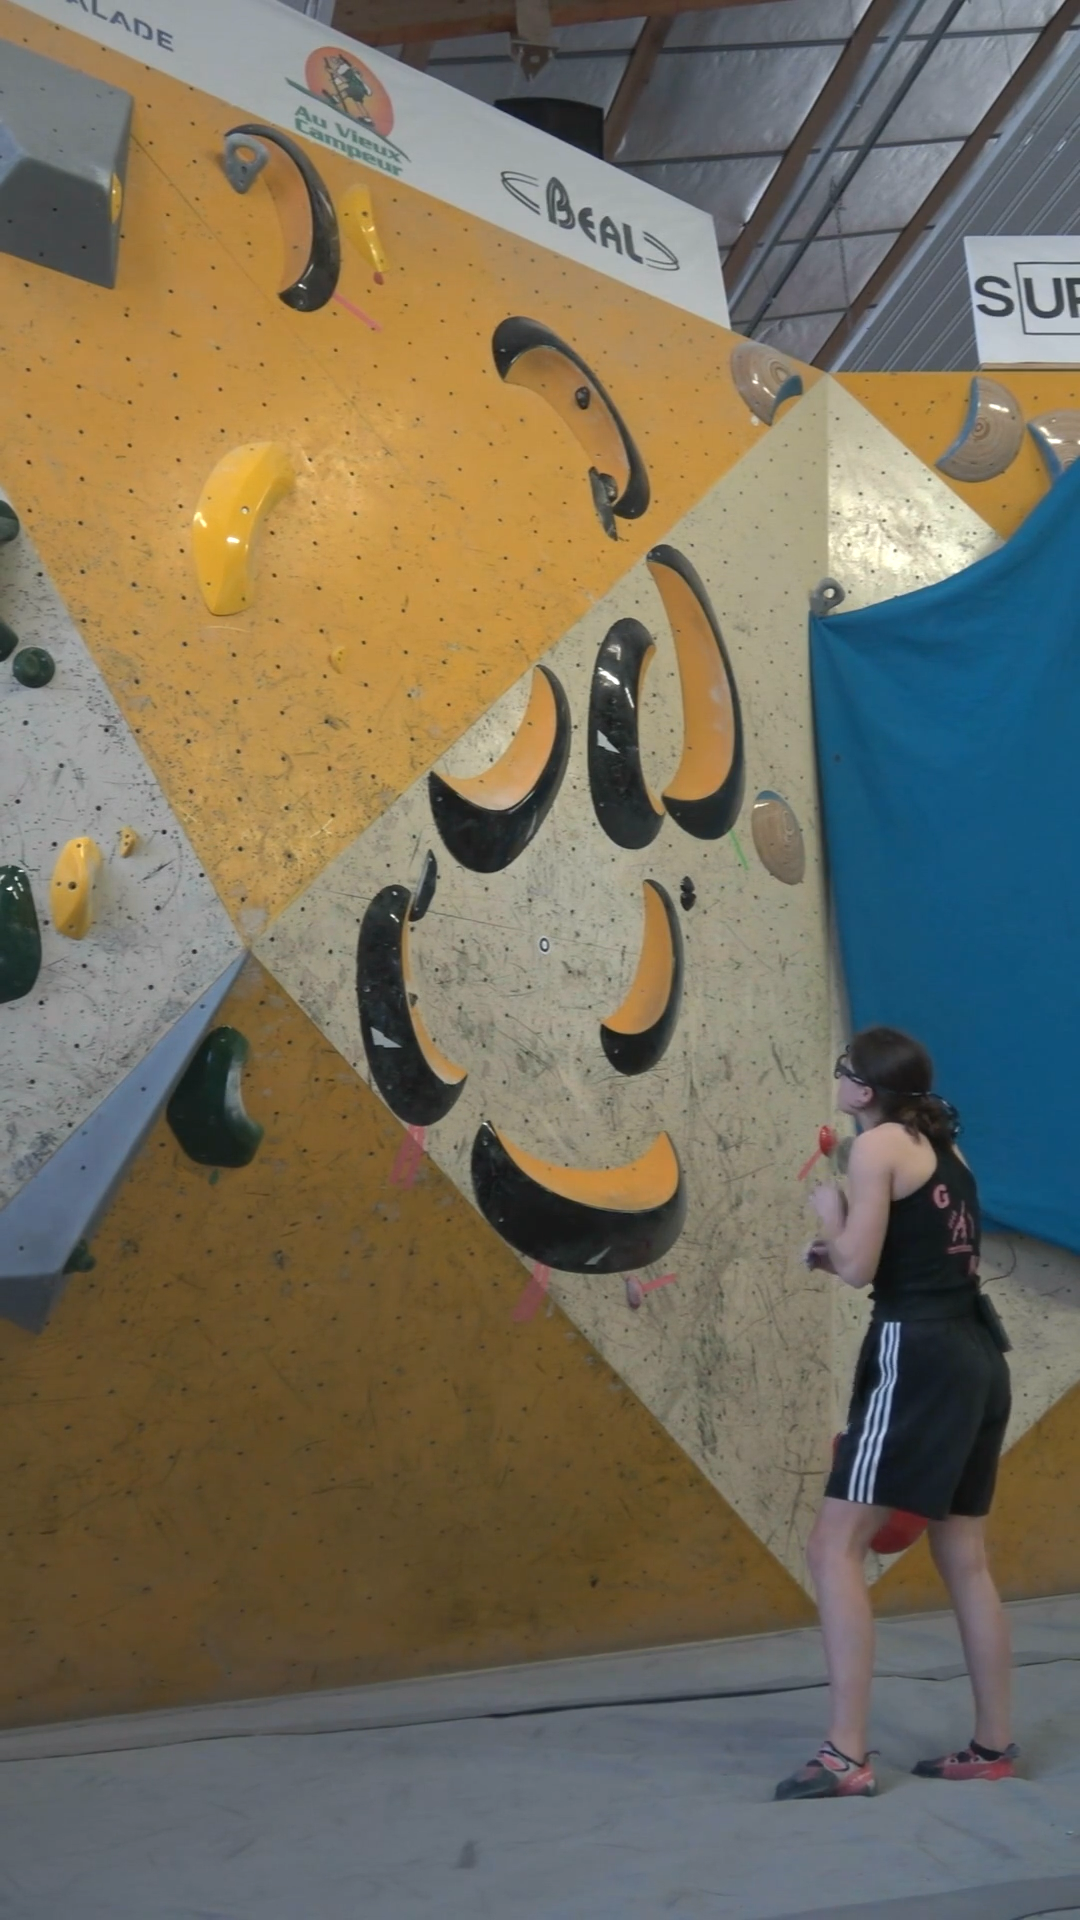
\includegraphics[width=0.2\textwidth]{assets/images/observing.2.png}} &
      \setlength{\fboxsep}{0pt}
      \fbox{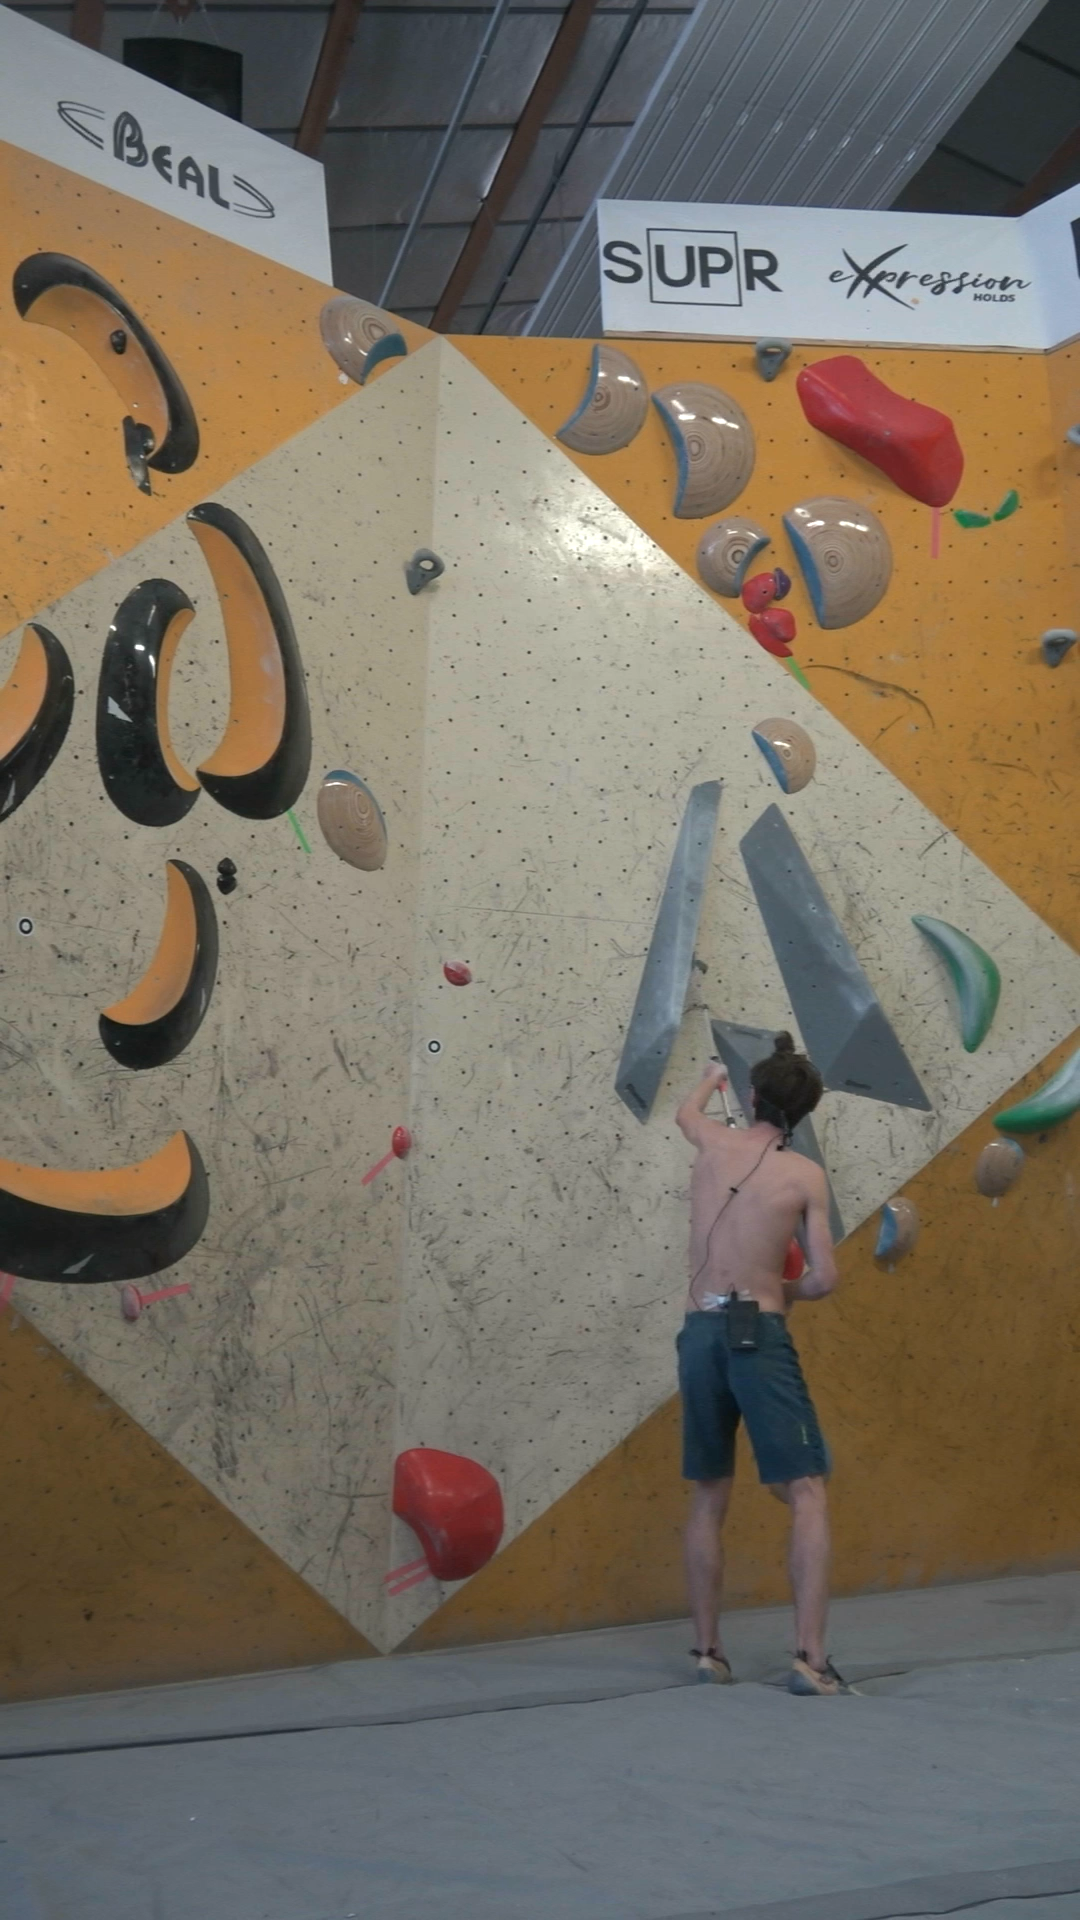
\includegraphics[width=0.2\textwidth]{assets/images/brushing.3.png}} &
      \setlength{\fboxsep}{0pt}
      \fbox{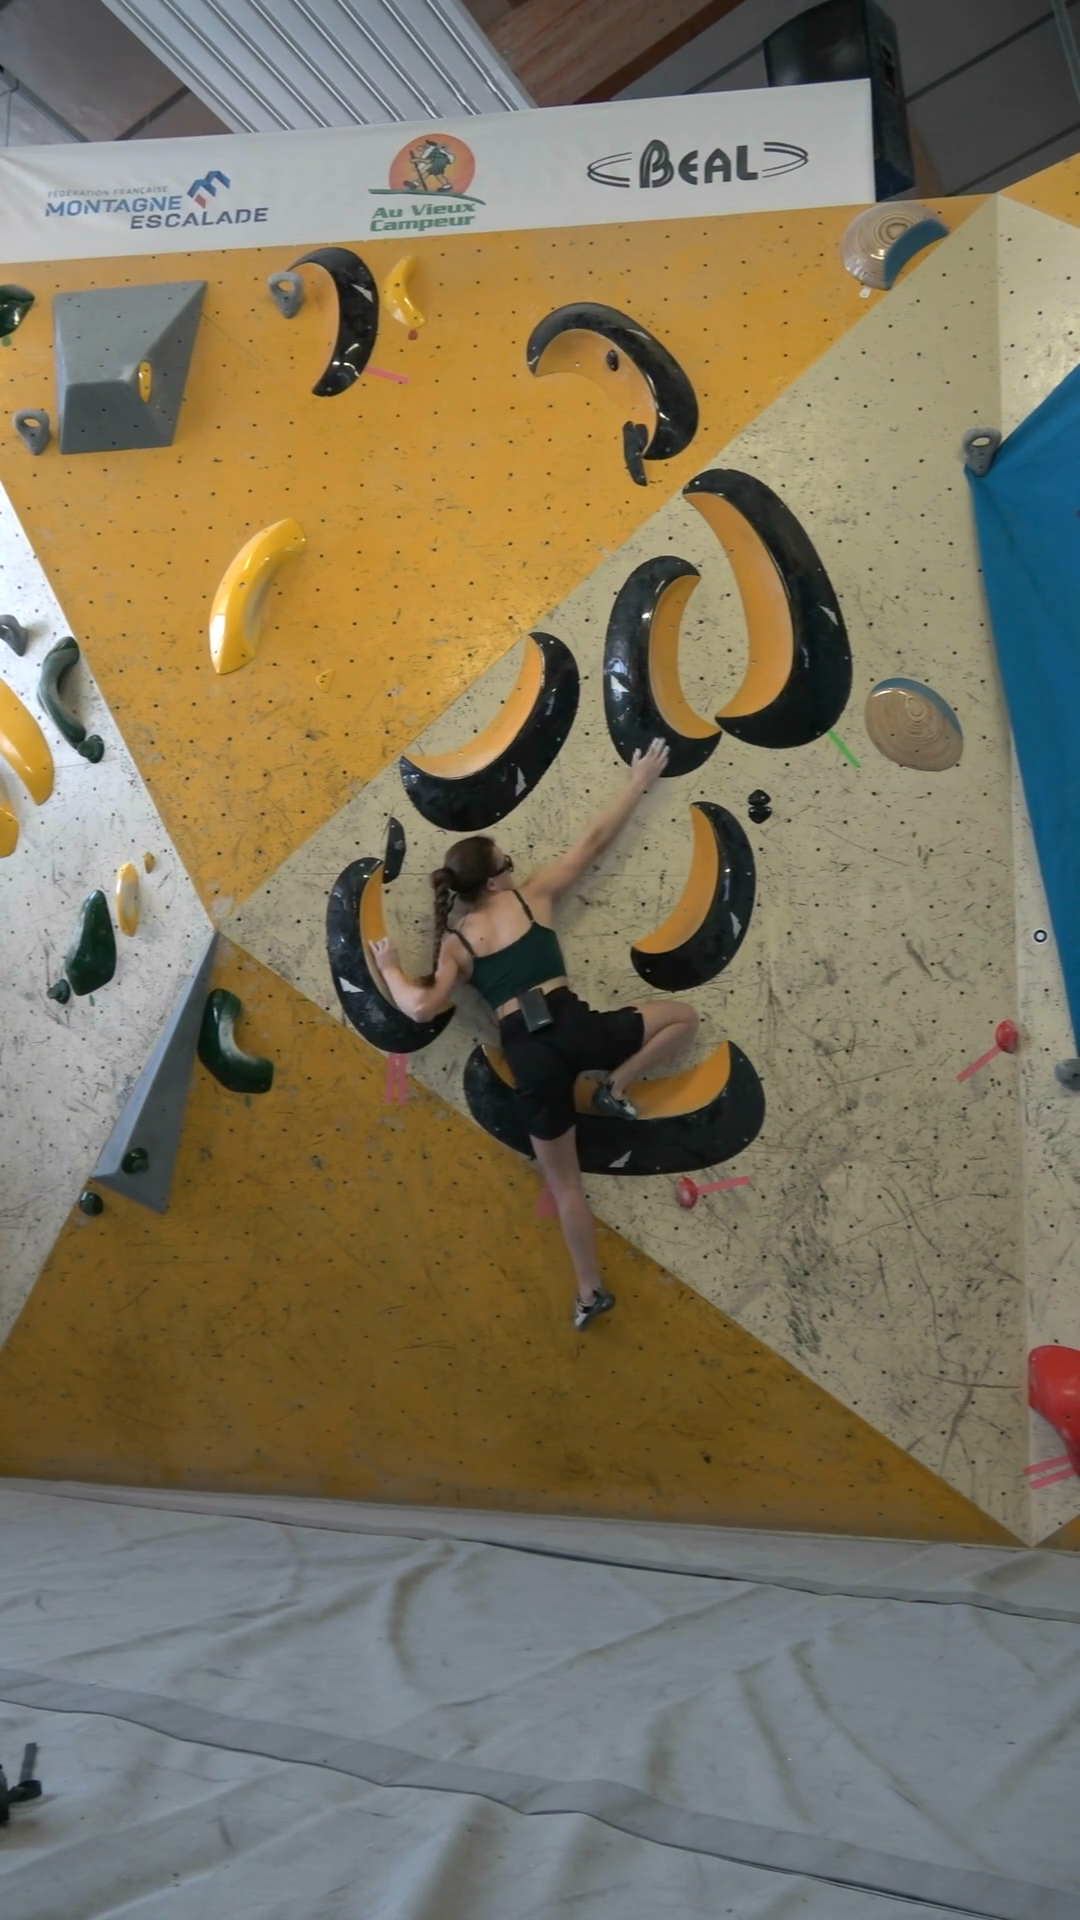
\includegraphics[width=0.2\textwidth]{assets/images/climbing.1.png}} &
      \setlength{\fboxsep}{0pt}
      \fbox{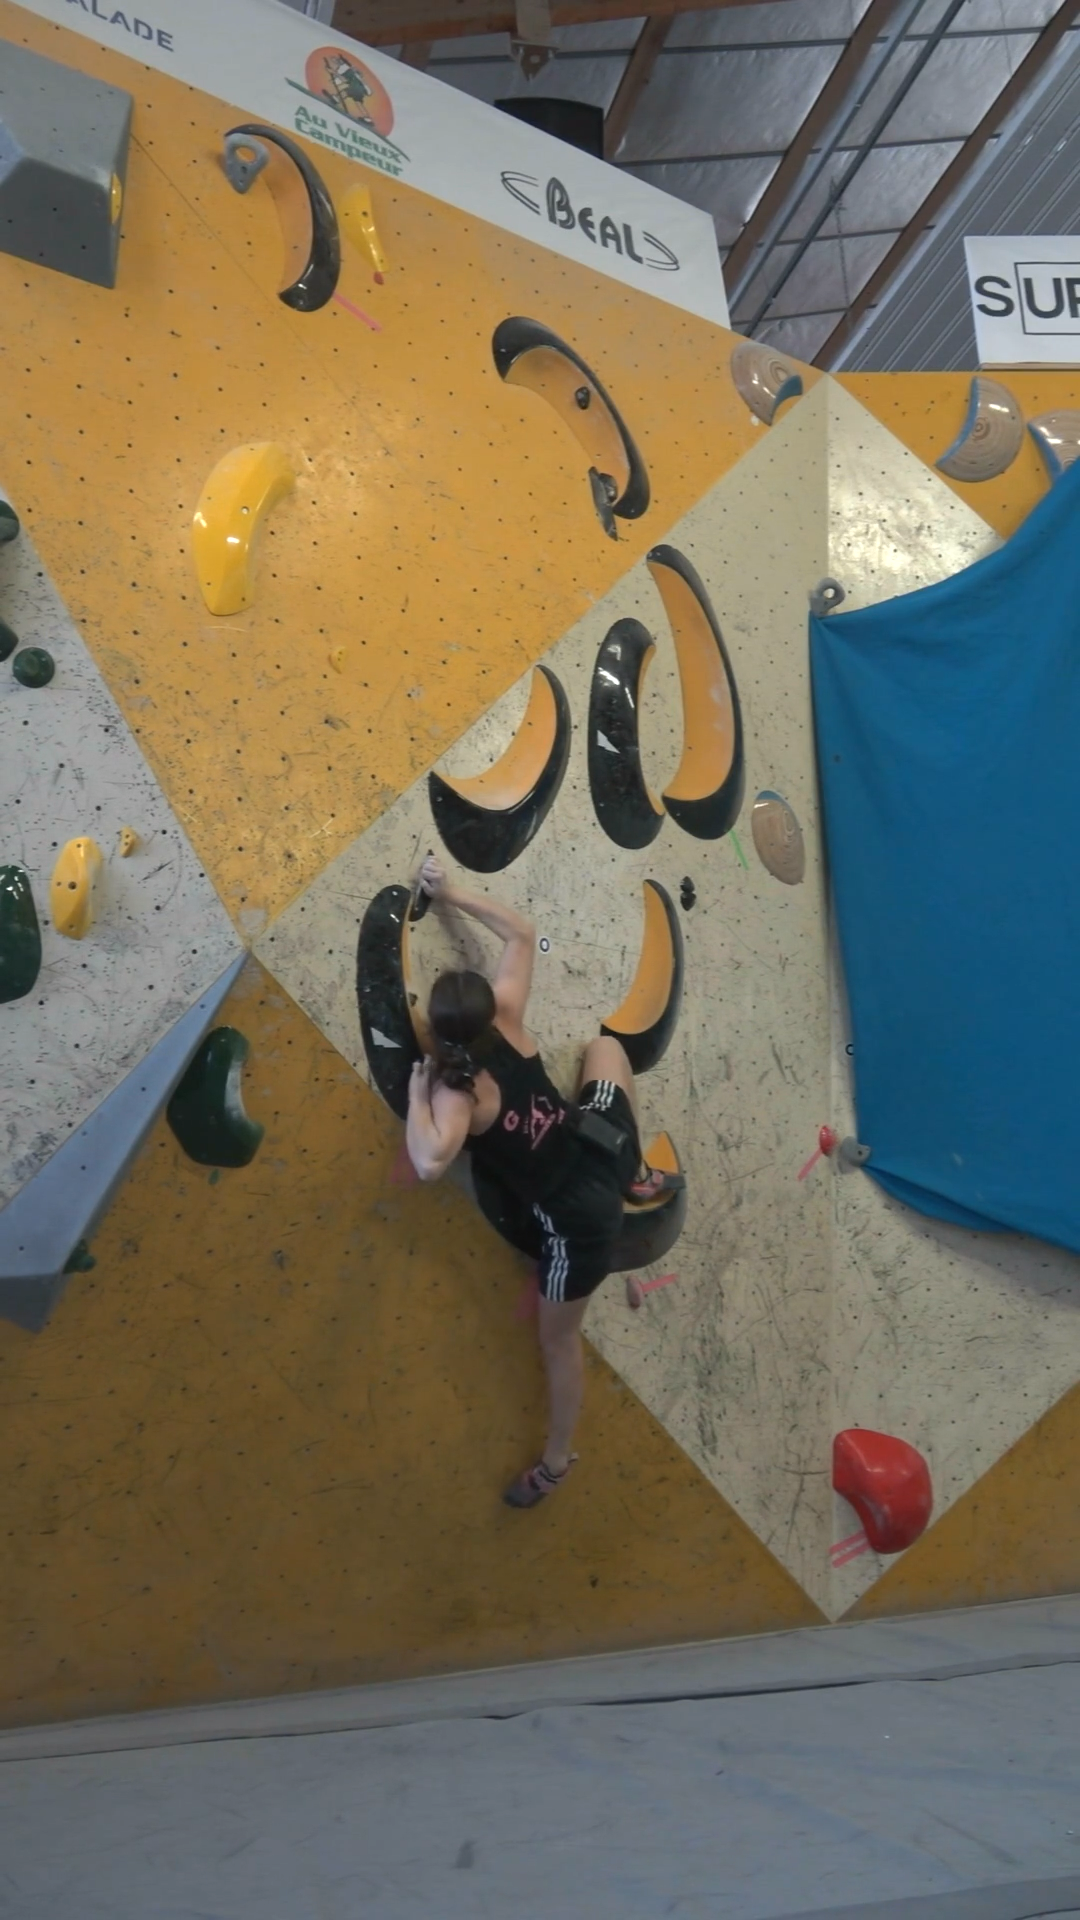
\includegraphics[width=0.2\textwidth]{assets/images/climbing.2.png}} \\[6pt]
      (a) Observing the block. &
      (b) Brushing the grips. &
      (c) Climbing the block. &
      (d) Climbing the block.
    \end{tabular}
    \caption{Different phases of bouldering.}
    \label{fig:phases-of-bouldering}
  \end{figure*}
\section{Objective}
\lipsum[1-2]
\section{Problem Presentation}
\lipsum[1-2]
\section{Dataset}
\lipsum[1-2]
\section{Popular Methods}

This will be a sort of state of the art.

Talk about the different approaches and techniques. Talk about their evolution just like it is done in \textbf{ViViT: A Video Vision Transformer} paper. (First started by using hand collected features, 2D CNNs, 3D with optical flow, full 3d, transformers as the datasets started to grow, etc.)

\lipsum[1-2]
\section{Our Approaches}
\lipsum[1-2]
\section{Other Paths to Explore}
\lipsum[1-2]
Talk about changing the loss, etc.
\section{Conclusion}

\subsection*{Research Contributions}
This work demonstrates the feasibility of automated bouldering video segmentation using modern deep learning approaches. Our experiments revealed that segment-based models, particularly the X3D family and the R3D, outperform frame-based approaches for this task, achieving accuracies of up to 86.80\%. We established that the choice of pre-training dataset significantly impacts performance, as evidenced by the stark difference between S3D models trained on HowTo100M versus Kinetics. Notably, model complexity did not necessarily correlate with performance, with lighter models often matching or exceeding their larger counterparts.

Future research should focus on improving real-time capabilities, investigating alternative loss functions, and exploring transformer-based architectures for video understanding. Semi-supervised approaches leveraging unlabeled climbing footage could address the data scarcity challenge while maintaining evaluation integrity.

\subsection*{Project Reflection}
This project provided valuable experience in end-to-end data science development. Building a computer vision system from scratch presented numerous challenges, from data collection and annotation to model selection and evaluation. The need to balance performance requirements against computational constraints mirrors real-world AI deployment scenarios.

The most significant challenge was navigating the vast landscape of video understanding models without extensive training resources. This required careful consideration of transfer learning approaches and creative solutions for data augmentation.

This work served as a formative experience in independent research, requiring comprehensive exploration of the computer vision literature and adaptation of techniques across domains. It demanded proficiency across the entire machine learning pipeline—from data preparation to deployment considerations—providing practical skills beyond what typical structured projects offer. This holistic approach to solving a complex visual understanding problem has reinforced both technical capabilities and research methodology fundamentals.

\begin{tcolorbox}[colback=lightgray!10, colframe=black, title={Research Aim}]
    Our goal is to \textit{demystify long chain-of-thought reasoning} in LLMs. Through systematic analysis and ablations, we extract key insights and offer practical strategies to enhance and stabilize its performance.
\end{tcolorbox}
\vspace{-10pt}

\section*{Acknowledgment}
Thanks to \lipsum[10].

\listoftodos

\bibliography{reference}
\bibliographystyle{icml2025}

\newpage
\appendix
\onecolumn
% You can have as much text here as you want. The main body must be at most $8$ pages long.
% For the final version, one more page can be added.
% If you want, you can use an appendix like this one.  

% The $\mathtt{\backslash onecolumn}$ command above can be kept in place if you prefer a one-column appendix, or can be removed if you prefer a two-column appendix.  Apart from this possible change, the style (font size, spacing, margins, page numbering, etc.) should be kept the same as the main body.

\section{Related Work}
\paragraph{Complex reasoning and chain of thought prompting.} Large Language Models (LLMs) have demonstrated remarkable capabilities in various natural language processing tasks, including complex reasoning. A significant advancement in improving LLM reasoning ability is the implementation of Chain of Thought (CoT) prompting \cite{wei2022cot}. This technique involves guiding models to generate intermediate reasoning steps, thereby improving their performance on tasks that require logical deduction and multistep problem solving. Initial studies \cite{lambert2024tulu, wei2022cot, flan, yu2024metamath} focused on short CoT, where models produce concise reasoning paths to arrive at solutions. Although effective for straightforward problems, short CoT can be limiting when addressing more intricate tasks that necessitate deeper deliberation. OpenAI’s o1 \cite{openai2024o1} series models were the first to introduce inference-time scaling by increasing the length of the CoT reasoning process. This approach helps LLMs tackle complex problems by breaking them into finer steps and reflecting during problem-solving, leading to more accurate and comprehensive solutions. In this work, we explore long CoT by identifying key factors that enable models to exhibit this behavior, encouraging advanced reasoning capabilities.

\paragraph{Reinforcement learning for LLM.} Reinforcement Learning (RL) has proven effective in enhancing LLM performance across domains. RL techniques, such as Reinforcement Learning from Human Feedback (RLHF), align model outputs with human preferences, improving coherence \cite{ouyang2022training}. Recent studies \cite{kimi2025k15, deepseekai2025r1, lambert2024tulu} leverage RL to enable LLMs to explore reasoning paths autonomously for complex problems. DeepSeek-R1 \cite{deepseekai2025r1} achieves strong performance in mathematics, coding, and reasoning tasks without relying on a trained reward model \cite{lightman2023verifystep, wang2024multistep} or tree search \cite{feng2023alphazerolike, snell2024scaling}. Notably, this capability emerges even in base models without supervised fine-tuning, albeit at the cost of output readability. Similarly, Kimi K1.5 \cite{kimi2025k15} enhances general reasoning with RL, focusing on multimodal reasoning and controlling thought process length. These works highlight RL’s role in optimizing reasoning when intermediate steps are hard to supervise, and only final outcomes are verifiable. Our research share a similar setup but with more detail on disentangling how different model behaviors emerge under varying training conditions and initialization strategies.

\newpage
\section{Figures and Tables}

%\begin{figure}[H]
%    \centering
%    \includegraphics[width=1\linewidth]{figs/viz-judge-rule.pdf}
%    \vspace{-20pt}
%    \caption{Downstream task performance when trained on clean data}
%    \label{fig:reward-verifier-clean}
%\end{figure}

\begin{table}[H]
\small
\caption{Performance of model trained with different discount factors for the correctness (cosine) reward and repetition penalty. We see that different reward types have different optimal values.}
\vspace{10pt}
\centering
\begin{tabular}{@{}cccccc@{}}
\toprule
\begin{tabular}[c]{@{}c@{}}Correctness \\ Discount\end{tabular} & \begin{tabular}[c]{@{}c@{}}Repetition\\ Discount\end{tabular} & \begin{tabular}[c]{@{}c@{}}MATH\\ -500\end{tabular} & \begin{tabular}[c]{@{}c@{}}AIME \\ 2024\end{tabular} & \begin{tabular}[c]{@{}c@{}}Theo.\\ QA\end{tabular} & \begin{tabular}[c]{@{}c@{}}MMLU\\ -Pro-1k\end{tabular} \\ \midrule
\multicolumn{2}{c}{SFT} & 50.4 & 3.5 & 20.6 & 32.4 \\ \midrule
\multirow{3}{*}{1.000} & 1.000 & 55.7 & \textbf{5.0} & 25.7 & 34.5 \\
 & 0.999 & \textbf{58.0} & 4.6 & \textbf{26.0} & \textbf{36.5} \\
 & 0.99 & 57.8 & 3.8 & 24.5 & 33.3 \\ \midrule
\multirow{2}{*}{0.999} & 0.999 & 53.5 & 2.1 & 19.5 & 30.7 \\
 & 0.99 & 55.2 & 1.7 & 18.5 & 32.0 \\ \midrule
0.99 & 0.99 & 47.9 & 0.2 & 15.6 & 25.5 \\ \bottomrule
\end{tabular}%
\label{fig:multiple-gamma}
\end{table}

\newpage
\section{Algorithms and Formulas}

\subsection{Cosine Reward Formula}

\begin{equation}
\label{eqn:cosine-lr}
\textbf{CosFn}(t, T, \eta_{min}, \eta_{max}) = \eta_{min} + \frac{1}{2}(\eta_{max} - \eta_{min})(1 + \cos(\frac{t\pi}{T}))
\end{equation}

The formula above is commonly used as the learning rate schedule during gradient descent optimization. It was introduced by \cite{loshchilov2017sgdrstochasticgradientdescent}.

\subsection{N-gram Repetition Penalty}

\begin{algorithm}[H]
\caption{N-gram Repetition Penalty}\label{alg:reward-repetition-penalty}
\begin{algorithmic}[1]
    \STATE {\bfseries Input:} 
    \STATE \ \ \ \ $s$ : sequence of tokens
    \STATE \ \ \ \ $l$ : sequence length
    \STATE \ \ \ \ $N$ : n-gram size
    \STATE \ \ \ \ $P$ : penalty value
    \STATE \ \ \ \ $m$ : maximum sequence length
    \STATE {\bfseries Output:} $r \in \mathbb{R}^m$
    \STATE $seq \gets s[1:l]$ \COMMENT{Extract subsequence of length $l$}
    \STATE $ngrams \gets \emptyset$ \COMMENT{Set of observed n-grams}
    \STATE $r \gets \vec{0} \in \mathbb{R}^m$ \COMMENT{Initialize reward vector}
    \FOR{$j \gets 1$ to $|seq| - N + 1$}
        \STATE $ng \gets (seq[j], seq[j+1], ..., seq[j+N-1])$ \COMMENT{Current n-gram}
        \IF{$ng \in ngrams$}
            \FOR{$t \gets j$ to $j + N - 1$}
                \STATE $r[t] \gets P$ \COMMENT{Apply penalty}
            \ENDFOR
        \ENDIF
        \STATE $ngrams \gets ngrams \cup \{ng\}$
    \ENDFOR
    \STATE {\bfseries Output:} $r$
\end{algorithmic}
\end{algorithm}

\newpage
\section{Extracts}

\begin{tcolorbox}[label=extract:reward-short-term, colback=lightgray!10, colframe=black, title={Short-Term Thinking ($\gamma_c = 0.99$)}]
\textbf{But} in this case, we saw that the fixed points don't satisfy the equation 
\[
p(p(x)) = x.
\]

\textbf{Wait}, maybe the solutions to \( p(p(x)) = x \) are not the fixed points of \( p \), but something else.

\textbf{Alternatively}, perhaps I can consider that \( p(p(x)) = x \) implies that \( p \) is a bijection, 
but since \( p(x) \) is quadratic, it's not necessarily invertible over all real numbers.

\textbf{Wait}, but the problem says that \( p(p(x)) = x \) has four real solutions, so perhaps there are four 
values of \( x \) that satisfy this equation.

\textbf{Alternatively}, perhaps I need to find the roots of 
\[
p(p(x)) - x = 0,
\]
and solve for \( x \). But that seems complicated. Maybe there's a better way.
\end{tcolorbox}

\newpage
\section{Experimental Setup}

\subsection{Evaluation Setup} \label{app:eval-setup}

\paragraph{Benchmarks} Below are details of our evaluation benchmarks:

\begin{itemize}
    \item \textbf{MATH-500} \citep{hendrycks2021math}: an in-domain mathematical reasoning benchmark. MATH consists of 12,500 problems from American high school math competitions. For efficiency, we adopt MATH-500, a widely-used i.i.d. subset of its test split.
    \item \textbf{AIME 2024}: an out-of-domain mathematical reasoning benchmark consisting of the 30 problems from American Invitational Mathematics Examination (AIME) 2024.
    \item \textbf{TheoremQA} \citep{chen2023theoremqa}: an out-of-domain STEM reasoning benchmark consisting of 800 samples. It covers 350+ theorems spanning across Math, EE\&CS, Physics and Finance.
    \item \textbf{MMLU-Pro-1k} \citep{wang2024mmlupro}: an out-of-domain general reasoning benchmark. MMLU-Pro comprises over 12,000 questions from academic exams and textbooks, spanning 14 diverse domains including Biology, Business, Chemistry, Computer Science, Economics, Engineering, Health, History, Law, Math, Philosophy, Physics, Psychology, and Others. For efficiency, we adopt an 1,000-sample i.i.d. subset of its test split, called MMLU-Pro-1k. We tried to keep the distribution identical to the original one. Figure \ref{fig:mmlu-pro-test-downsample} shows the distribution before/after the downsampling.
\end{itemize}

\paragraph{Statistical Metrics} We calculate the average accuracy with at least 4 random seeds. To tame the variance caused by the small size of AIME 2024, we sample 16 responses per prompt.


\end{document}

